%!TEX root = ../main.tex
%=========================================================

\section{Introduction}
With an average of 23,500 constantly live nodes~\cite{discv4-dns-lists}, Ethereum is one of the largest decentralized platforms currently in operation.
While it is widely known for supporting the blockchain of the same name (also known as the \emph{mainnet}), the Ethereum platform is also home to a number of additional decentralized applications.
This includes blockchains used for test purposes (\emph{Ropsten}, \emph{G\"orli}), divergent blockchains resulting from a past fork (\emph{Ethereum classic}), alternative cryptocurrencies (\emph{Pirl}, \emph{Musicoin}), exchange markets (\emph{Binance}), content delivery networks (\emph{Swarm}), or messaging applications (\emph{Whisper}).
The platform already features almost 500 applications, and their number grows every year~\cite{discv4-dns-lists}. The size distribution of the application-specific sub-networks varies significantly (\Cref{fig:ecosystem}) featuring a \emph{long tail}, with a vast majority of applications formed of a few hundred nodes or less.

\begin{figure}[t]
    \includegraphics[width=1\linewidth]{img/ecosystem}
    % \vspace{-2mm}
    \caption{Distribution of the number of nodes in Ethereum's sub-networks, corresponding to different applications (May 2022).
    Sub-networks are sorted by decreasing popularity.
    A Zipf distribution is given for reference.
    }
    \label{fig:ecosystem}
\end{figure}

All nodes in the Ethereum platform participate in a \emph{global} peer-to-peer (P2P) network operating a distributed hash table (DHT)~\cite{maymounkov2002kademlia}.
In addition to joining the global network, every node connects to at least one \emph{sub-network} formed of peers participating in its application(s) of interest.
In this paper, we focus on the \emph{service discovery} mechanism, by which a node participating in the global P2P network discovers an application sub-network.
This mechanism returns a set of peers that are used as entry points to the P2P overlay specific to that application, as illustrated by \Cref{fig:subnetwork}.

\begin{figure}[b!]
    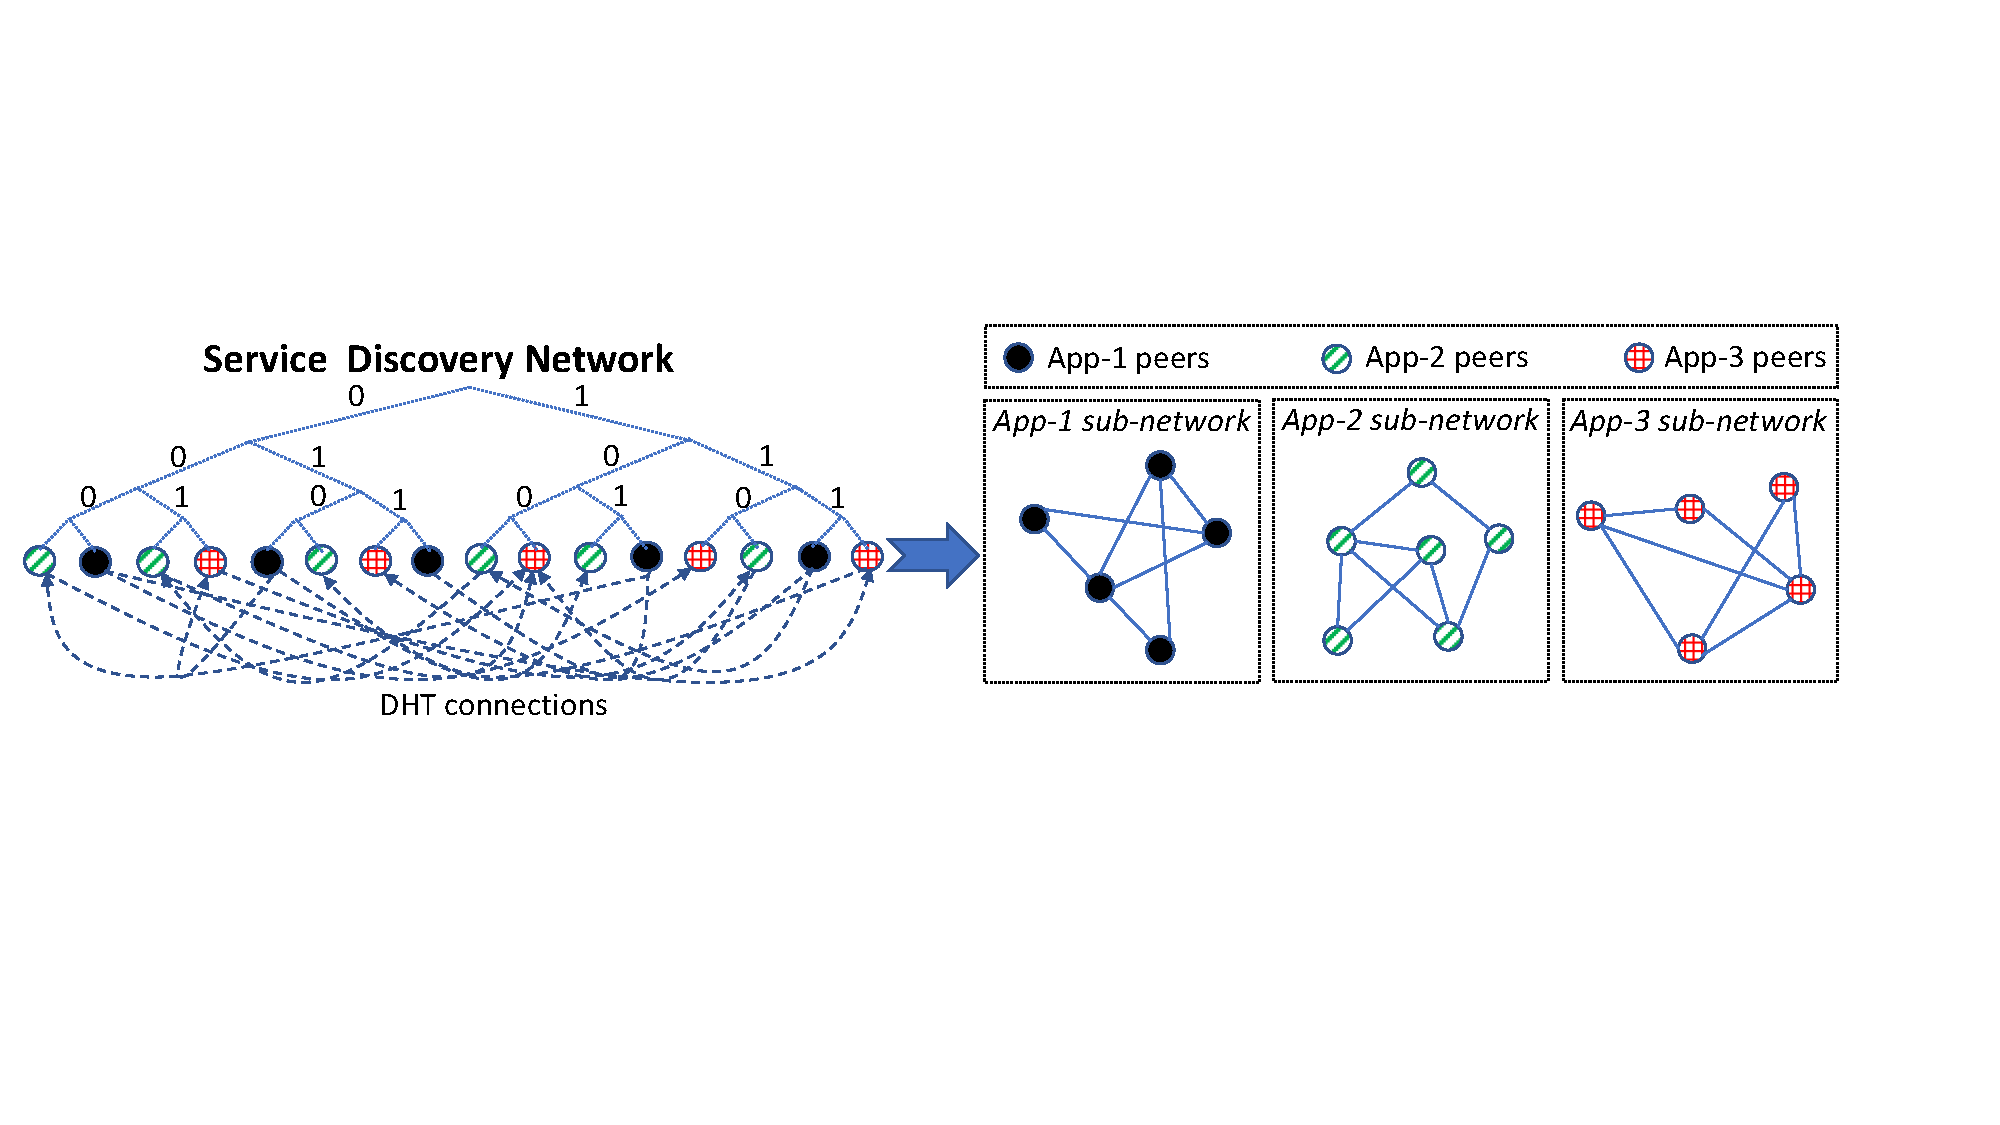
\includegraphics[width=1\linewidth]{img/subnetwork}
    \caption{Formation of application-specific sub-networks using a universal service discovery network.
    }
    \label{fig:subnetwork}
\end{figure}

Service discovery is a particularly sensitive mechanism in the Ethereum platform.
It must ensure that malicious participants to this open network are unable to bias its execution against a victim node or sub-network--and that, despite the ability of these adversaries to operate multiple Sybil identities.
Of particular importance is the protection against \emph{eclipse} attacks, where an adversary would lure its victim(s) into a sub-network formed of only nodes under its control.
Similarly, an adversary may run \emph{denial-of-service} attacks against a specific application, preventing other nodes from discovering peers from the associated sub-network.
On the other hand, the mechanism must remain efficient and scalable.
It is not desirable, in particular, that it relies solely on a fixed set of dedicated registrar nodes maintaining the membership of each application, both for scalability and robustness reasons. Registrar nodes for popular applications could quickly become overwhelmed, and be an easy target for attackers.
In addition, the need to provision dedicated registrar nodes would be a hindrance to the emergence of new applications and (initially) small sub-networks.


The current service discovery mechanism used in the Ethereum platform is part of \discv~\cite{discv4}, a set of protocols leveraging the global DHT.
It employs a simple but robust \emph{random walk} approach.
A node willing to join an application's sub-network simply contacts individually a series of nodes collected from random lookups on the DHT, repeatedly checking application membership until it has collected enough peers participating in this target application.
This approach offers good resilience to malicious behaviors but it suffers from very poor scalability and performance, in particular for small sub-networks.
As more applications join the DHT, the inefficiency of the random discovery process becomes a bottleneck for the entire ecosystem. While alternative solutions for service discovery have been proposed, they are meant for small-scale network~\cite{zhang2002aggregate, helal2002standards}, centralised~\cite{RFC6763}, based on unrealistic assumptions~\cite{danezis2005sybil, danezis2009sybilinfer} or insecure~\cite{baldoni2007tera,scribe,poldercast,banno2015,scribe}. We provide an extensive analysis of these systems in \Cref{sec:related}.

\smallskip
\noindent
\textbf{Contributions.}
%
We detail in this paper \sysname, a novel service discovery mechanism for large-scale, decentralized platforms and its application to Ethereum.
\sysname targets a balance between robustness, i.e., the ability to resist malicious behaviors and Sybil identities, efficiency, i.e., fast service discovery even for small applications, and good load-balance over participating nodes.

After providing background knowledge and reviewing the current service discovery mechanism of Ethereum in \Cref{sec:background}, and detailing our system and thread models in \Cref{sec:model}, we detail \sysname as follows.

In \Cref{sec:placement}, we present how this new protocol enables nodes, members of application sub-networks, to \emph{advertise} their membership to these applications in the form of \emph{service advertisements}.
Any node can act as a \emph{registrar} and store advertisements for any topic.
In contrast with the direct use of the DHT as a key-value store, however, in \sysname service advertisements propagate to a pseudo-random subset of all nodes in the global network.
The density of advertisements for an application increases as a DHT lookup approaches its associated key in the DHT overlay structure.

Robustness, load balancing, and efficiency for the discovery of smaller sub-networks all rely on a novel \emph{admission protocol}, by which registrars accept or reject incoming service advertisements (\Cref{sec:admission}).
It ensures that advertisers cannot effectively flood advertisements at a registrar even when deviating from the protocol or operating Sybils and that less popular topics get a sufficiently high probability to be represented and looked up.

At the core of our novel admission protocol lies the need for registrants to respect a waiting time imposed by the registrars before being able to successfully register their advertisement.
We discuss the design and dynamics of the waiting function in \Cref{sec:waitingTime}.
The function allows limiting the amount of resources used by each node, promotes diversity of topic advertisements stored by each node, and protects against a vast range of malicious behaviors.


We overcome multiple practical challenges, implement \sysname in a simulator as well as in the code base of \emph{discv5}~\cite{discv5} (\ie, Node Discovery protocol version 5) - a new set of P2P protocols replacing \emph{discv4}~\cite{discv4}. 
%We intend to release the full code and dataset of our experiment open source with the unblinded version of this paper.
\hl{Our results show ...}
\sysname already has two full-stack industrial implementations and is scheduled for deployment in the future versions of Ethereum.